\section{Kernel construction for convolutions}

\subsection{Simple case with $r=2$ error correction cycles}

\subsection{Representation of measure qubit state changes when $r\geq 3$}


%%%%%%%%%%%%%%%%%%%%%%%%%%%%%
\begin{figure*}[htb]
\centering
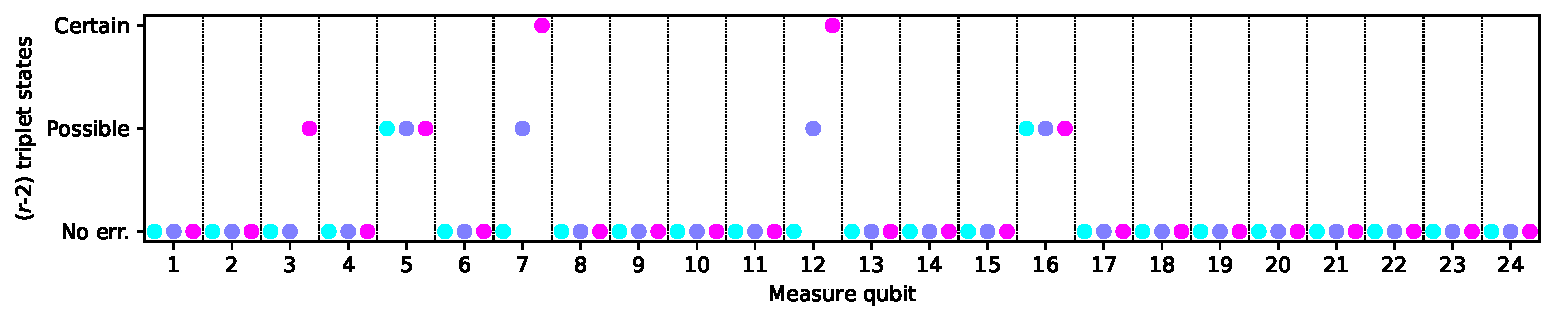
\includegraphics[width=0.9\textwidth]{states_d5_r5_event0.pdf} \\
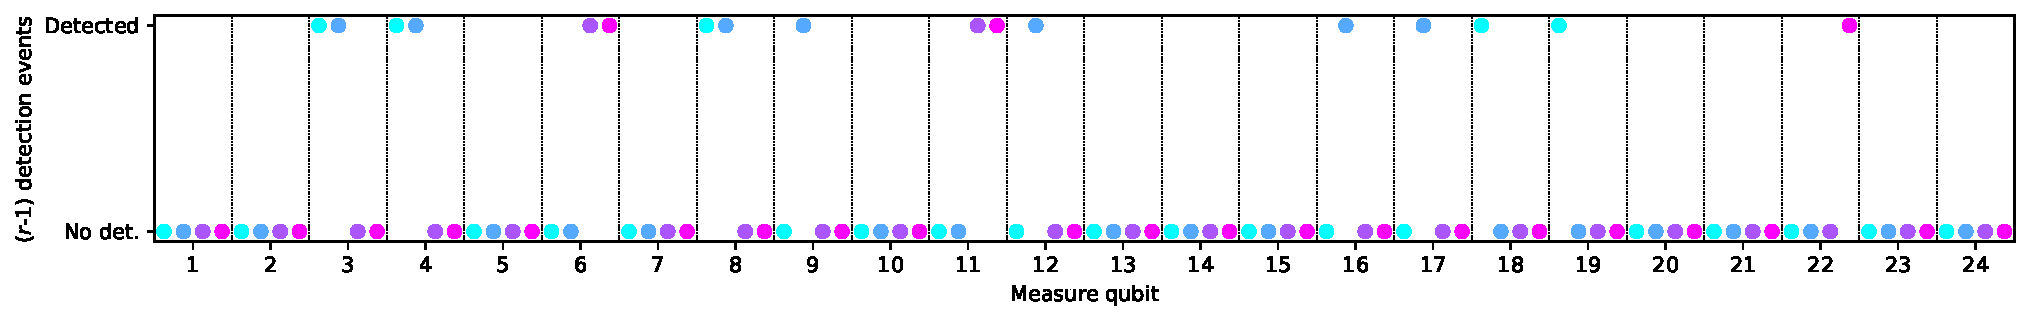
\includegraphics[width=0.9\textwidth]{det_evts_d5_r5_event0.pdf}
\ccaption
{Measure qubit raw states and detection events for $d=5$, $r=5$}
{
}
\label{fig:d5r5states}
\end{figure*}
%%%%%%%%%%%%%%%%%%%%%%%%%%%%%



\subsection{Recurrent convolutional kernel architecture for $r\geq 3$}
